\documentclass[tikz,border=10pt]{standalone}
% no extra packages beyond TikZ; no libraries needed for this figure
\begin{document}
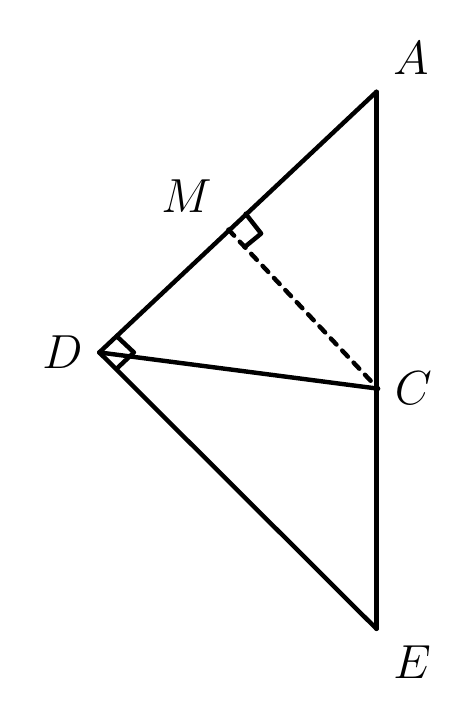
\begin{tikzpicture}[line width=1.6pt, line join=round, line cap=round]
  % Points (pixel -> units, s = 0.01995, y flipped, centre (145,222))
  \coordinate (A) at (1.76,3.41);
  \coordinate (E) at (1.76,-3.41);
  \coordinate (D) at (-1.76,0.10);
  \coordinate (C) at (1.78,-0.36);
  \coordinate (M) at (-0.12,1.66);

  % Solid segments
  \draw (A) -- (D);
  \draw (A) -- (E);
  \draw (D) -- (E);
  \draw (D) -- (C);

  % Dashed segment M to C
  \draw[dashed] (M) -- (C);

  % Right-angle mark at M (between MA and MC)
  \draw (0.099,1.861) -- (0.2955,1.61) -- (0.0855,1.438);

  % Right-angle mark at D (between DA and DE, as listed in the GES)
  \draw (-1.538,0.305) -- (-1.320,0.100) -- (-1.538,-0.105);

  % Labels
  \fontsize{16}{19.2}\selectfont
  \node[above right] at (A) {$A$};
  \node[below right] at (E) {$E$};
  \node[left] at (D) {$D$};
  \node[right] at (C) {$C$};
  \node[above left] at (M) {$M$};
\end{tikzpicture}
\end{document}